\documentclass[a4paper, 12pt]{article}

%%% SST LAB PROTOCOLL PREAMBLE
%%% 2019
%%%%%%%%%%%%%%%%%%%%%%%%%%%%%%%


%%% PACKAGES
%%%%%%%%%%%%%%%%%%%%%%%%%%%

\usepackage[ngerman]{babel}

\usepackage[utf8]{inputenc}
\usepackage{amsmath}
\usepackage{pgfplots}
\usepackage{tikz}
\usepackage[many]{tcolorbox}
\usepackage{graphicx}
\graphicspath{ {./graphics/} }
\usepackage{pdfpages}
\usepackage{dashrule}
\usepackage{float}
\usepackage{siunitx}
\usepackage{booktabs}
\usepackage[version=4]{mhchem}

%%% DOCUMENT GEOMETRY
%%%%%%%%%%%%%%%%%%%%%%%%%%%

\usepackage{geometry}
\geometry{
 a4paper,
 total={0.6180339887498948\paperwidth,0.6180339887498948\paperheight},
 top = 0.1458980337503154\paperheight,
 bottom = 0.1458980337503154\paperheight
 }
\setlength{\jot}{0.013155617496424828\paperheight}
\linespread{1.1458980337503154}

\setlength{\parskip}{0.013155617496424828\paperheight} % paragraph spacing


%%% COLORS
%%%%%%%%%%%%%%%%%%%%%%%%%%%

\definecolor{red1}{HTML}{f38181}
\definecolor{yellow1}{HTML}{fce38a}
\definecolor{green1}{HTML}{95e1d3}
\definecolor{blue1}{HTML}{66bfbf}
\definecolor{hsblue}{HTML}{00b1db}
\definecolor{hsgrey}{HTML}{afafaf}

%%% CONSTANTS
%%%%%%%%%%%%%%%%%%%%%%%%%%%
\newlength{\smallvert}
\setlength{\smallvert}{0.0131556\paperheight}


%%% COMMANDS
%%%%%%%%%%%%%%%%%%%%%%%%%%%

% differential d
\newcommand*\dif{\mathop{}\!\mathrm{d}}

% horizontal line
\newcommand{\holine}[1]{
  	\begin{center}
	  	\noindent{\color{hsgrey}\hdashrule[0ex]{#1}{1pt}{3mm}}\\%[0.0131556\paperheight]
  	\end{center}
}

% mini section
\newcommand{\minisec}[1]{ \noindent\underline{\textit {#1} } \\}

% quick function plot
\newcommand{\plotfun}[3]{
  \vspace{0.021286\paperheight}
  \begin{center}
    \begin{tikzpicture}
      \begin{axis}[
        axis x line=center,
        axis y line=center,
        ]
        \addplot[draw=red1][domain=#2:#3]{#1};
      \end{axis}
    \end{tikzpicture}
  \end{center}
}

% box for notes
\newcommand{\notebox}[1]{

\tcbset{colback=white,colframe=red1!100!black,title=Note!,width=0.618\paperwidth,arc=0pt}

 \begin{center}
  \begin{tcolorbox}[]
   #1 
  \end{tcolorbox}
 
 \end{center} 
 
}

% box for equation
\newcommand{\eqbox}[2]{
	
	\tcbset{colback=white,colframe=hsblue!100!black,title=,width=#2,arc=0pt}
	
	\begin{center}
		\begin{tcolorbox}[ams align*]
				#1
		\end{tcolorbox}
		
	\end{center} 
	
}

% END OF PREAMBLE

%%%%%%%%%%%%%%%%%%%%%%%%%%%%%%%%%%%%%

\begin{document}

% 1
%%%%%%%%%%%%%%%%%%%%%%%%%%%%%%%%%%%%%
  
\includepdf{./titlepage/titlepage1.pdf}
  \clearpage
  \setcounter{page}{1}
%%%%%%%%%%%%%%%%%%%%%%%%%%%%%%%%%%%%%

\section{Vorbereitungsaufgaben}

\subsection{Funktion des Bipolartransistors}
\subsubsection{Spannungsgrenze}

\subsubsection{Leerlaufverstärkung}

\subsubsection{G}
-Ausgangsspannungsgrenze
-Leerlaufverstärkung
-CMRR, Gleichtakt/Gegentaktverstärkung
-Eingangsruheströme
-Gleichtakteingwiderstand differenzeingwiderstand

\subsection{Vierquadrantenkennlinienfeld}
\begin{figure}[H]
  \begin{center}
    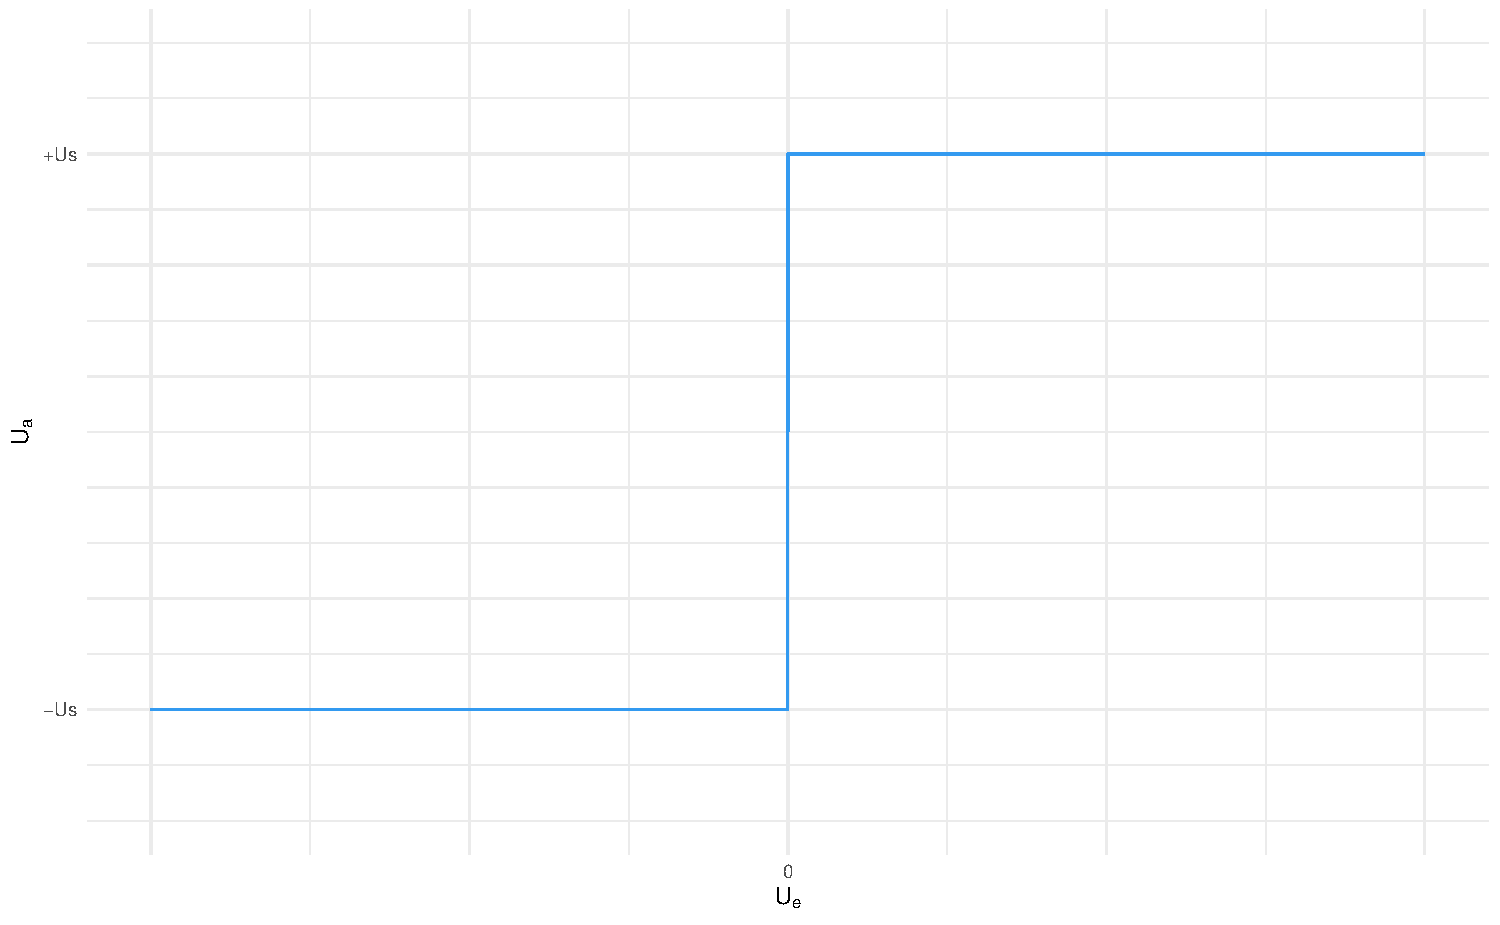
\includegraphics[width=0.618\textwidth]{1_2/opv_nofeed.pdf}
    \end{center}
    \caption{OPV-Kennlinie ohne Rückkopplung (ideal)}
 \end{figure}
\begin{figure}[H]
  \begin{center}
    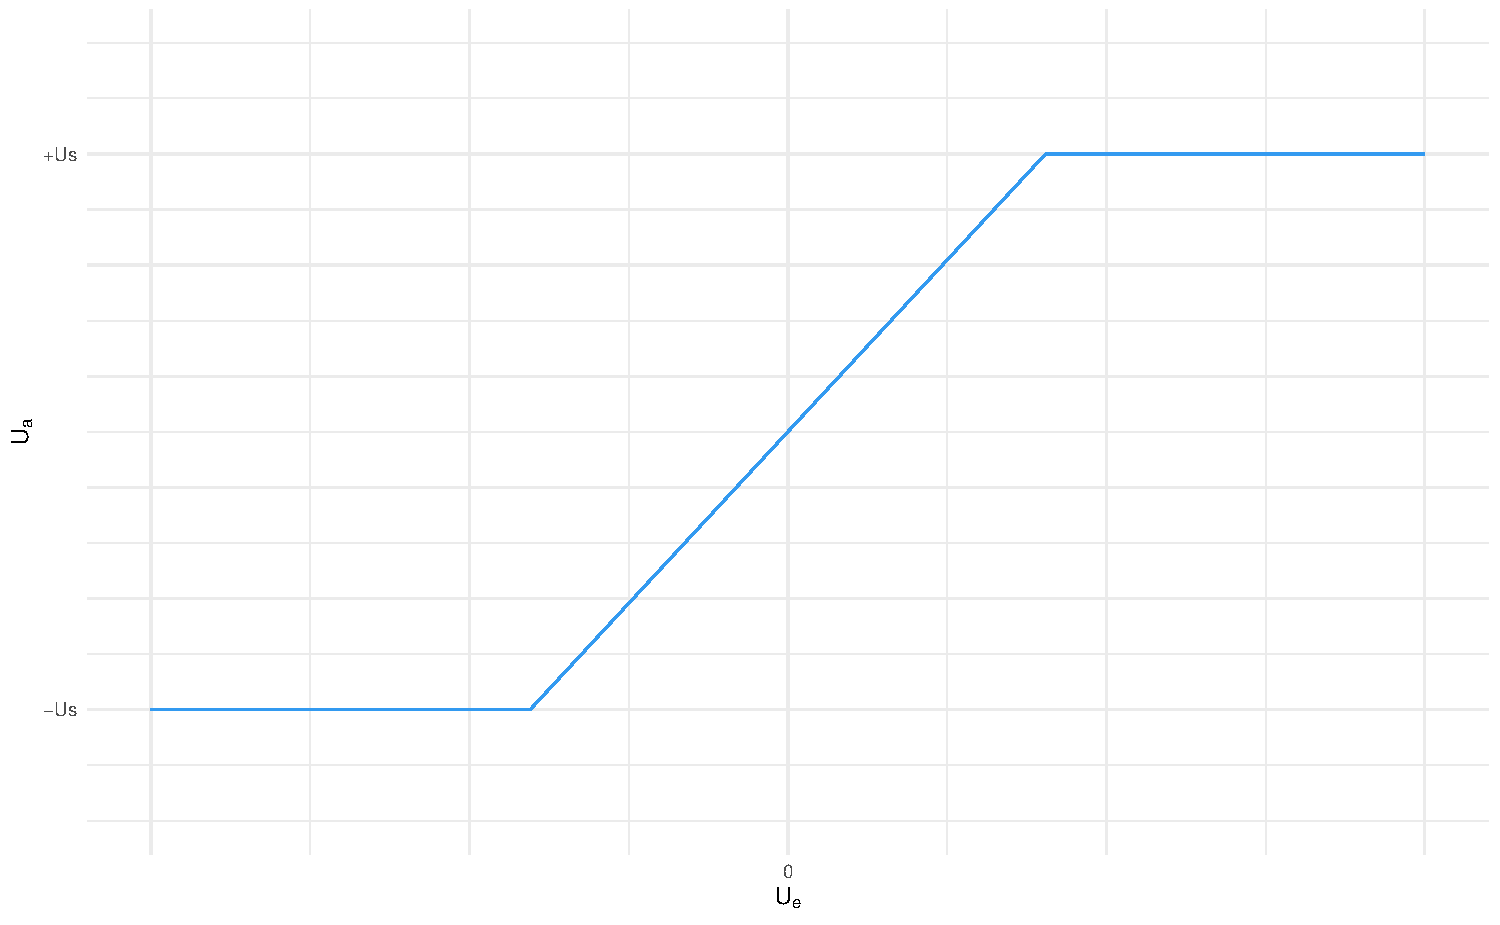
\includegraphics[width=0.618\textwidth]{1_2/opv_feed.pdf}
    \end{center}
    \caption{OPV-Kennlinie mit Rückkopplung}
 \end{figure}

Durch Rückführung eines Teils des Ausgangs- auf das Eingangssignal durch ein
Rückkopplungsnetzwerk wird der Operationsverstärker in einen linearen
Arbeitsbereich gebracht, wodurch die Verstärkung nicht mehr den Wert der der Leerlaufverstärkung (Abb. 1), sondern einen kontrollierten Verstärkungswert (Abb. 2) annimmt.


\subsection{Vierpolersatzschaltbild}
  \begin{figure}[H]
\begin{center}
    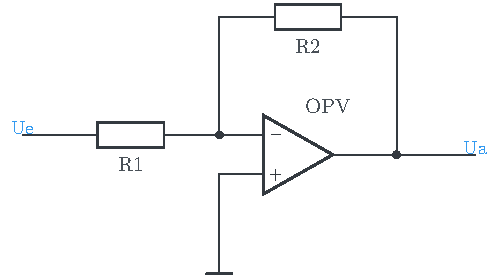
\includegraphics[width=0.618\textwidth]{circuits/inv_verst.pdf}
\end{center}
    \caption{Invertierende Verstärkerschaltung}
  \end{figure}

\begin{gather*}
  U_a = V_0(U_p-U_n)\\
  U_p = 0 \, \si{\volt}\\
  U_a = -V_0 \cdot U_n\\
  \intertext{Bestimmung von $U_n$ durch Überlagerung der Eingangs- und
    Ausgangswirkung:}
  U_n = U_n' + U_n''\\
  U_n' = U_n|_{U_a=0}\\
  = U_e \cdot \frac{R_2}{R_1 + R_2}\\
  U_n'' = U_n|_{U_e=0}\\
  = U_a \cdot \frac{R_1}{R_1 + R_2}\\
  U_a = -V_0 \cdot U_e \cdot \frac{R_2}{R_1+R_2} - V_0 \cdot U_a \cdot
  \frac{R_1}{R_1+R_2}\\
  U_a (1 + V_0 \cdot \frac{R_1}{R_1+R_2}) = -V_0 \cdot U_e \cdot \frac{R_2}{R_1+R_2}\\
  \frac{U_a}{U_e} = V = - \frac{V_0 \cdot \frac{R_2}{R_1+R_2}}{1+V_0 \cdot
    \frac{R_1}{R_1+R_2}} = - \frac{V_0}{(R_1+R_2) + V_0 \cdot R_1}\\
  V = - \frac{R_2}{\frac{R_1+R_2}{V_0} + R_1}\\
  \intertext{für $V_0 \rightarrow \infty$}
  V = -\frac{R_2}{R_1}
\end{gather*}

\subsection{Transistorgrundschaltungen}
\begin{figure}[H]
  \begin{center}
    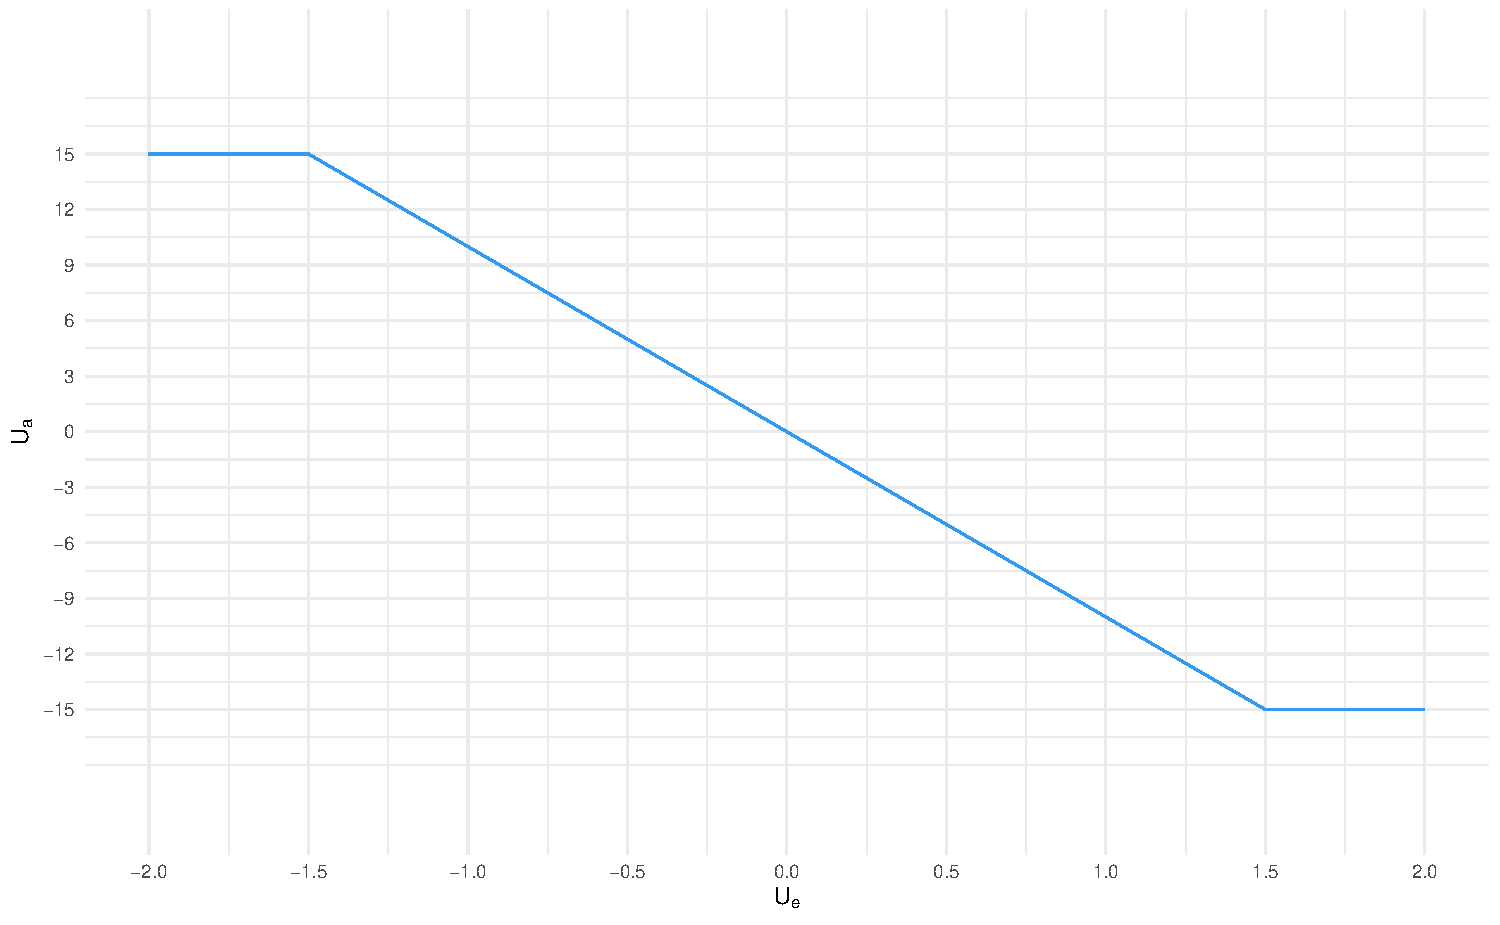
\includegraphics[width=\textwidth]{1_4/opv_inv_verst.pdf}
    \end{center}
    \caption{Kennlinie eines (idealen) OPV mit einer Verstärkung von $V_u = -10$ und einer
      Versorgungsspannung von $U_s = \pm 15 \, \si{\volt}$}
 \end{figure}


\subsection{Dimensionierung einer Emitterstufe}
Die Spannung über dem Emitterwiderstand $U_{R_4}$ wird gewählt
\[ U_{R_4} = 1 \, \si{\volt}\]

\noindent Damit ergibt sich die Spannung $U'$ am Basisspannungsteiler zu
\[ U' = 1 \, \si{\volt} + 0.7 \, \si{\volt} = 1.7 \, \si{\volt}\]

Der Querstrom durch den Spannungsteiler wird so hoch gewählt, dass dieser
bezüglich des Basisstroms als unbelastet angesehen werden kann. 
\[I_{R_1} = 8 \cdot I_B\]

\noindent Der Basisstrom
\[I_B = \frac{I_C}{\beta} = \frac{4.5 \, \si{\milli\ampere}}{158} = 27.22 \, \si{\micro\ampere}\]

\noindent führt zu den Widerstandswerten des Basisspannungsteilers
\[R_2 = \frac{U'}{8 \cdot I_B} = \frac{1.7 \, \si{\volt}}{8 \cdot 27.22 \,
    \si{\micro\ampere}} = 7.87 \, \si{\kilo\ohm}\]

\[R_1 = \frac{U_s - U'}{9 \cdot I_B} = \frac{10.3 \, \si{\volt}}{244.98 \,
    \si{\micro\ampere}} = 42.2 \, \si{\kilo\ohm}\]

Die verbleibenden Widerstände sind
\[ R_4 =  \frac{U_{R_4}}{I_{C,A}} = \frac{1 \, \si{\volt}}{4.3 \,
    \si{\milli\ampere}} = 232 \, \si{\ohm}\]

\[R_3 = \frac{U_s - U_{R_4} - U_{CE,A}}{I_{C,A}} = \frac{5 \, \si{\volt}}{4.3 \,
  \si{\milli\ampere}} = 1.15 \, \si{\kilo\ohm}\]

Die Widerstandswerte wurden so gerundet, dass sie jeweils in eine E-Reihe passen.

Der Kondensator parallel zu $R_3$ kann so gewählt werden, dass seine Reaktanz $X_C$ bei der
niedrigsten Signalfrequenz gleich $1/10\, R_3$ ist.

\subsection{Temperaturabhängigkeiten}
Temperaturänderungen stellen für den Transistor als Halbleiterbauelement eine
externe Energiezufuhr und damit eine Störung des thermodynamischen
Gleichgewichts dar. Die Ladungsträgerdichten der einzelnen Bereiche
erhöhen sich, die Weiten der Raumladungszonen verringern sich und der Transistor
wird insgesamt leitfähiger. Dadurch erhöht sich auch der
Stromverstärkungsfaktor $\beta$, was z.B. den Arbeitspunkt, der bei der
Schaltungsdimensionierung angenommen wurde, verschieben kann. Da dieser zusätzlich
fertigungsbedingt abweichen kann, strebt man einen
Arbeitspunkt an, der möglichst unabhängig von der Stromverstärkung ist. Dies
wird z.B. durch die Arbeitspunkteinstellung mit einem 4-Widerstandsnetzwerk oder
die Einstellung des Emitterstroms durch eine Stromquelle erreicht.



\subsection{Bestimmung der Grundschaltungsparameter}
\begin{gather*}
  r_{\mathrm{ein}} = \frac{U_e}{I_e} \\
  \intertext{virtuelle Masse, daher $I_e = I_{R_1}$, $U_{R_1} = U_e$ }
  r_{\mathrm{ein}} = \frac{U_e}{I_{R_1}} = \frac{U_e}{\dfrac{U_e}{R_1}}\\
  r_{\mathrm{ein}} = R_1\\
\end{gather*}

\subsection{Messtechnische Bestimmung der Ein- und Ausgangsparameter}
\subsubsection{Bestimmung des Eingangswiderstands}
Allgemein gelingt die Widerstandsmessung indirekt durch eine Spannungs- und
Strommessung und anschließende Division der gemessenen Größen. 

\subsubsection{Bestimmung des Ausgangswiderstands}
Der Zusammenhang zwischen Lastwiderstand und Ausgangswiderstand des Verstärkers
ist linear (Zweipol)
\[R_a = \frac{U_{a,0} - U_{a,Last}}{I_{a,Last}}\]
\[R_a = \frac{U_{a,0} - U_{a,Last}}{U_{a,Last}} \cdot R_L\]
\[R_a = R_L \cdot \left(\frac{U_{a,0}}{U_{a,Last}}-1 \right)\]

Wobei $U_{a,0}$ die Leerlaufspannung am Ausgang, $U_{a,Last}$ die
Spannung am Ausgang bei Belastung mit dem Lastwiderstand $R_L$, und $R_a$ der
Ausgangswiderstand des Verstärkers ist.

Aus der Gleichung lässt sich erkennen, dass $R_a = R_L$ wenn $U_{a,Last} =
U_{a,0}/2$ ist. D.h. die Ausgangsspannung $U_{a,Last}$ kann bei
Belastung mit einem bekannten Lastwiderstandswert gemessen und anschließend in
der obigen Gleichung verwendet werden oder sie kann auf den halben Wert der
Leerlaufausgangsspannung durch einen variablen Lastwiderstand eingestellt
werden, wonach eine Messung des Lastwiderstandes folgt.


\subsubsection{Bestimmung der Verstärkungen}
Da die Verstärkungen frequenzabhängig sind und somit das Verhältnis von Ein- und
Ausgangsspannung (wechselspannungsmäßig) nicht konstant ist, muss man messtechnisch die
Übertragungsfunktion ermitteln, was beispielsweise durch das Durchlaufen mehrerer
Signalfrequenzen und anschließender Darstellung der
Ausgangsamplituden/-differenz erreicht werden kann (wobbeln). 

\subsection{Bootstrapschaltung}
\begin{figure}[H]
\begin{center}
  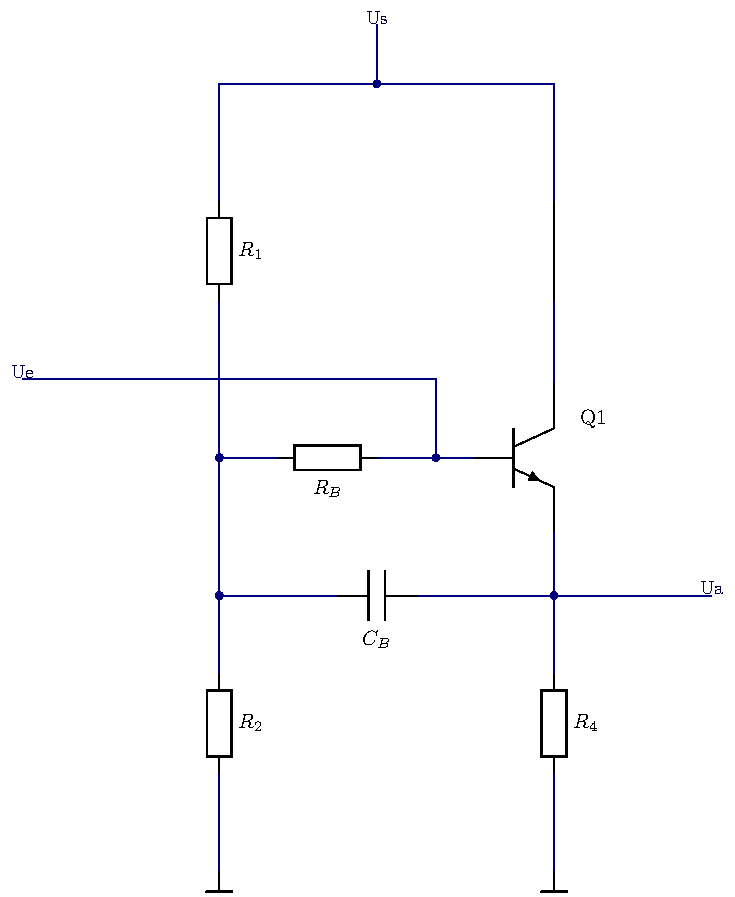
\includegraphics[width=0.618\textwidth]{circuits/bootstrap.pdf}
  \end{center}
\end{figure}


Bootstrapping ist eine Art der positiven Rückkopplung mit dem Ziel den
Eingangswiderstand der Schaltung zu erhöhen.

Bei der Kollektorschaltung kann
dies von Vorteil sein, um den Einsatz als Impedanzwandler zu verbessern.
Zur Kopplung wird ein Kondensator $C_B$ zwischen Ausgang und Basis geschaltet.
Eine schnelle Änderung des Ausgangssignals wirkt sich durch den Kondensator
ebenso auf den Eingang/die Basis aus, wobei beachtet werden muss, dass dieser so
dimensioniert ist, dass er bei der kleinsten Signalfrequenz einen Kurzschluss
darstellt.

Da die Verstärkung der Kollektorschaltung
kleiner als eins (z.B. 0.97) ist, beginnt der Verstärker nicht zu schwingen, wie es sonst
bei Mitkopplungen üblich wäre. Das Eingangssignal tritt mit leicht geringerer
Amplitude im Eingangskreis erneut auf, sodass der Strom durch den Widerstand
$R_B$, welcher den Basisspannungsteilerpunkt mit der Basis verbindet, sehr
gering ist, wodurch der scheinbare Wert von $R_B$ erhöht wird.

Der effektive (Kleinsignal-) Wert von $R_B$ ist
\[R_{B,eff} = \frac{R_B}{1-V_u}\]

\subsection{Frequenzverhalten}
Das Frequenzverhalten des Bipolartransistors wird durch die
Sperrschichtkapazität $C_{BC}$, welche im Normalbetrieb dominiert, sowie die
Diffusionskapazität $C_{BE}$ bestimmt, da diese im Ersatzschaltbild
frequenzabhängige Widerstände darstellen. 

\subsection{Grenzfrequenz und Bandbreite}
\begin{figure}[H]
  \begin{center}
    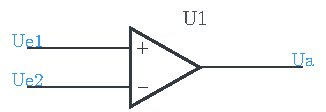
\includegraphics[width=0.618\textwidth]{circuits/komparator.pdf}
  \end{center}
  \caption{Einfache Komparatorschaltung}
\end{figure}

\[ U_a = V_0 (U_p - U_n) = V_0 (U_{e1} - U_{e2})\]

Ist $U_{e1}$ größer als $U_{e2}$ gerät der Operationsverstärker an seine
maximale positive Ausgangsspannung (idealerweise die
Versorgungsspannung), ist $U_{e1}$ kleiner als $U_{e2}$ an die maximal negative.
Legt man $U_{e2}$ auf einen konstanten positiven Referenzspannungswert, so verschiebt sich
die Kennline aus Abbildung 1 nach rechts.

\begin{figure}[H]
  \begin{center}
    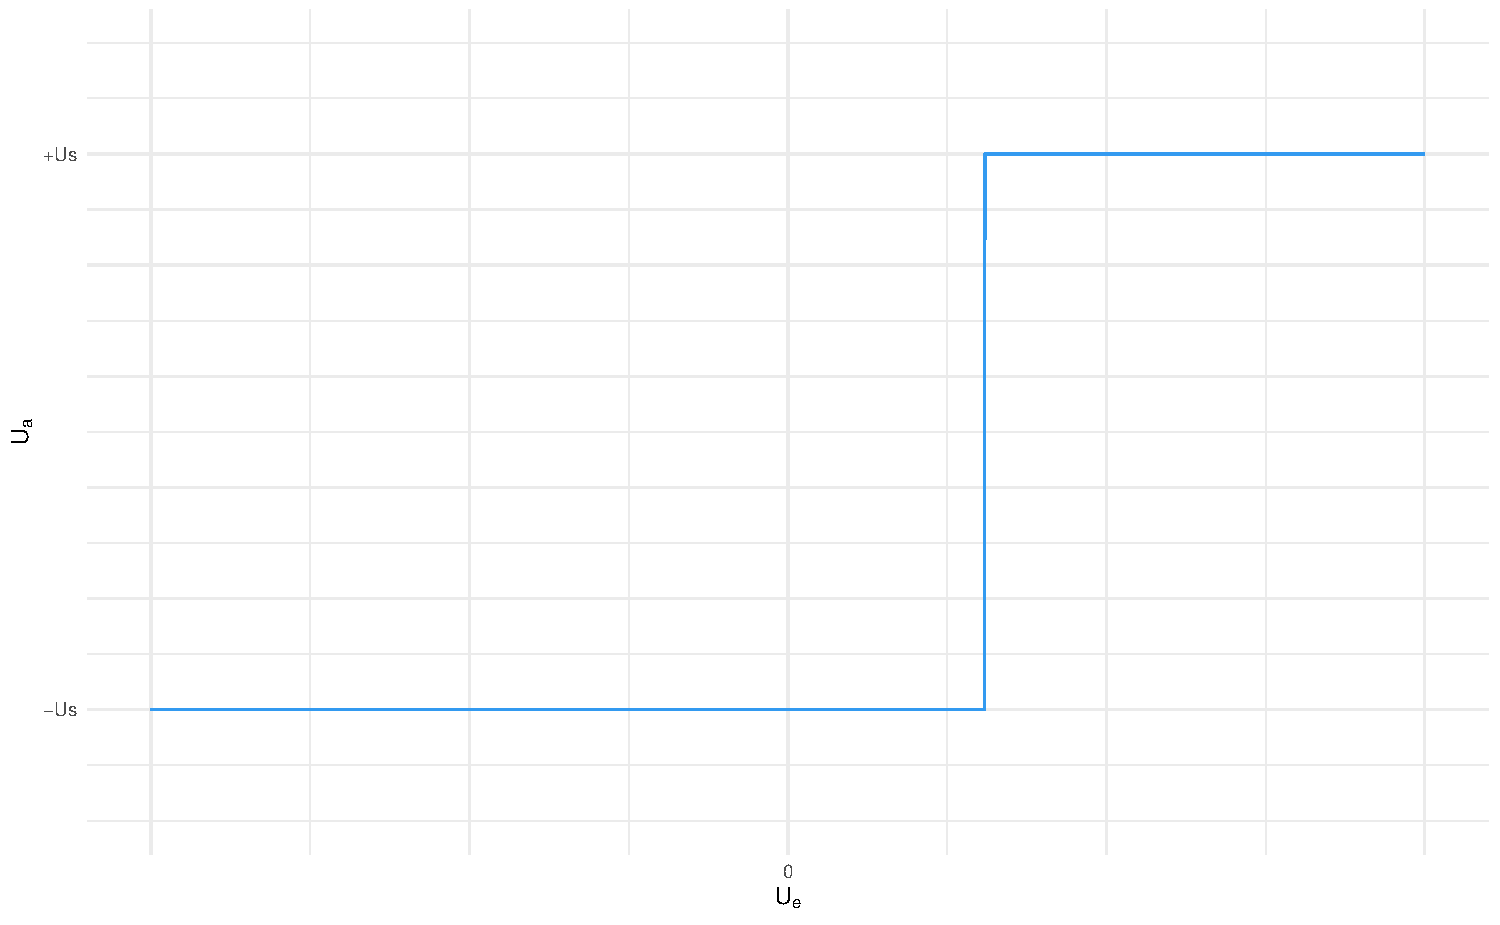
\includegraphics[width=\textwidth]{1_11/comparator.pdf}
  \end{center}
  \caption{Übertragungskennlinie der Komparatorschaltung mit positiver Referenzspannung ($U_{e2}$)}
\end{figure}


Zwischen invertierendem und nichtinvertierendem Eingang des
Operationsverstärkers können zwei Dioden antiparallel geschaltet werden, um die
Eingangsdifferenzspannung auf $\pm 0.7 \, \si{\volt}$ zu begrenzen. Zusätzlich
müssen dann zur Strombegrenzung Widerstände vor die Eingangs-/ Referenzspannung
geschaltet werden. 

\subsection{Millertheorem}
\begin{figure}[H]
  \begin{center}
    \includegraphics[width=\textwidth]{circuits/schmitt.pdf}
  \end{center}
  \caption{Schmitt-Trigger-Schaltung}
\end{figure}

\subsection{Grenzfrequenz der Emitterschaltung}
\begin{figure}[H]
  \begin{center}
    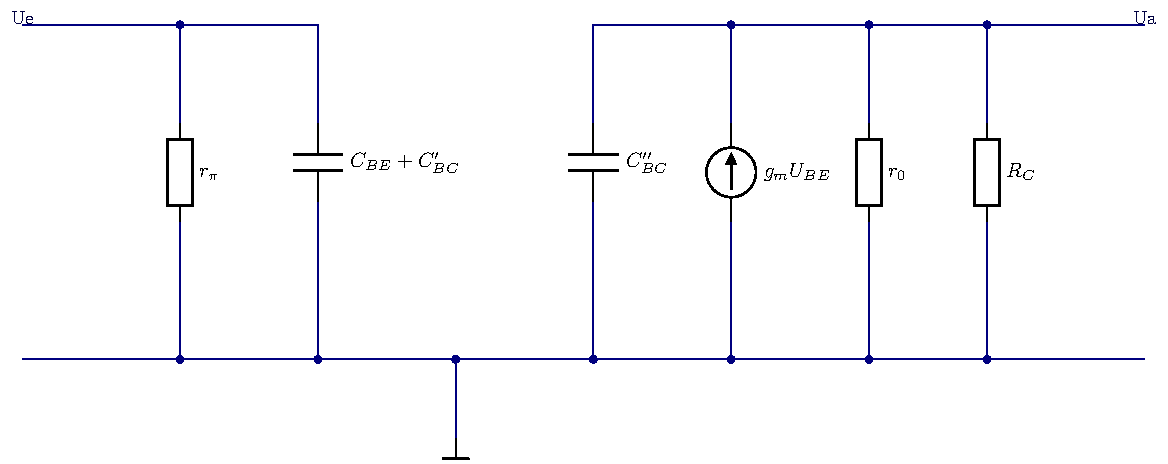
\includegraphics[width=0.618\textwidth]{circuits/commonEmitter_freq.pdf}
  \end{center}
  \caption{ESB der Emitterschaltung mit Millerkapazitäten}
\end{figure}

Die obere Grenzfrequenz der Schaltung wird durch die parasitären Kapazitäten des
Bipolartransistors bestimmt, die untere durch die Koppelkondensatoren der Schaltung

Eingangskreis:
\[0 = \frac{U_1}{r_\pi} + U_1 j \omega (C'_{BC}+C_{BE})-I_b\]

\noindent Ausgangskreis:
\[0 = g_m U_1 + \frac{U_a}{r_0 // R_C} - U_a j \omega C_{BC}''\]

\noindent Übertragungsfunktion
\[\frac{U_a}{U_e} = \frac{\frac{1}{r_\pi} +
    j\omega(C_{BC}'+C_{BE}) -g_m}{\frac{1}{r_0 // R_C} - j\omega C_{BC}''}\]

\noindent Grenzfrequenz
\[\omega_{gr} = \frac{1}{(C_{BE}+C_{BC}')r_\pi }\]

\[\left( \omega_{gr} = \frac{1}{(C_{BC}' + C_{BE})\cdot \frac{1}{g_m} - r_0
      C_{BC}''} \right) ? \]

% 2
%%%%%%%%%%%%%%%%%%%%%%%%%%%%%%%%%%%%%
  
\includepdf{./titlepage/titlepage2.pdf}
  \clearpage
  \setcounter{page}{1}
%%%%%%%%%%%%%%%%%%%%%%%%%%%%%%%%%%%%%

\section{Versuchsaufgaben} 

\setcounter{subsection}{1}
\subsection{Arbeitspunktbestimmung}
Die Ströme und Spannungen konnten teilweise nur indirekt gemessen werden und
mussten daher aus mehreren Messungen berechnet werden.

\subsubsection{ES\_IGK1}
Der Kollektorstrom $I_C$ der Schaltung wurde durch die Messung der Spannung über dem
Widerstand $R_3$ ($V_2 - U_C$)und entsprechender Division durch dessen Widerstandswert
ermittelt.
\[I_C  = \frac{V_2 - U_c}{R_3} = \frac{12.01 \, \si{\volt} - 6.38 \,
    \si{\volt}}{1.3 \, \si{\kilo\ohm}} = 4.33 \, \si{\milli\ampere}\]

Die Kollektorspannung konnte dann über Messung des Emitterpotentials $U_E$ gegen Masse
und Differenzbildung mit dem vorher bestimmten Wert $U_c$ bestimmt werden.
\[U_{CE} = U_C - U_E = 6.38 \, \si{\volt} - 0.436 \, \si{\volt} = 5.944 \, \si{\volt}\]

Der Basisstrom ist die Differenz aus dem Strom durch $R_1$ und dem Strom durch
$R_2$.
\[I_B = \frac{V_2 - U_B}{R_1}-\frac{U_B}{R_2} = \frac{12 \, \si{\volt} - 1.149
    \, \si{\volt}}{43 \, \si{\kilo\ohm}} - \frac{1.149 \, \si{\volt}}{5.1 \,
    \si{\kilo\ohm}} = 27.58 \, \si{\micro\ampere}\]

Die statische Stromverstärkung ist damit
\[B = \frac{I_C}{I_B} = \frac{4.33 \, \si{\milli\ampere}}{27.58 \,
    \si{micro\ampere}} = 157\]

Aus dem Datenblatt des 2N3904 Bipolartransistors lässt sich bei einem
Kollektorstrom vom etwa $I_C = 4 \, \si{\milli\ampere}$ und einer
Kollektor-Emitter-Spannung von $U_{CE} = 10 \, \si{\volt}$ ein
Stromverstärkungsfaktor von $B = 150$ ablesen. (Datenblatt onsemi Abb. 11).

\begin{figure}[H]
  \begin{center}
    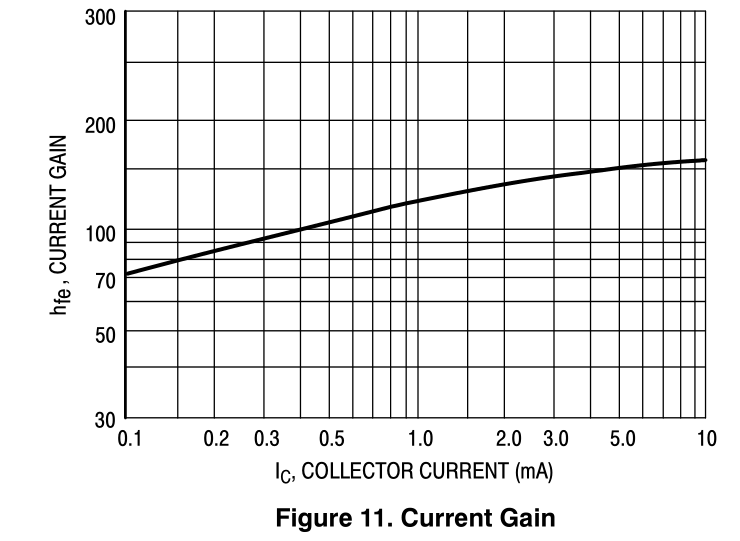
\includegraphics[width=0.618\textwidth]{2_2/ds1}
  \end{center}
  \caption{Quelle: http://onsemi.com}
\end{figure}

\subsubsection{ES\_IUGK1}
Die Arbeitspunktwerte der zweiten und dritten Schaltung wurden entsprechend 2.2.1 bestimmt.

\begin{table}[H]
\begin{center}
\begin{tabular}{c | c}
  $U_C$ & $6.06 \, \si{\volt}$\\
  \hline
  $U_E$ & $0.53 \, \si{\volt}$\\
  \hline
  $U_B$ & $1.23 \, \si{\volt}$\\
\end{tabular}
\end{center}
\caption{Zwischenwerte der Schaltung ES\_IUGK1}
\end{table}

\begin{table}[H]
\begin{center}
\begin{tabular}{c | c}
  $I_C$ & $5.23 \, \si{\milli\ampere}$\\
  \hline
  $U_{CE}$ & $5.53 \, \si{\volt}$\\
  \hline
  $I_{B}$ & $24.15 \, \si{\micro\ampere}$\\
  \hline
  $B$ & $216 $\\
\end{tabular}
\caption{Arbeitspunktwerte der Schaltung ES\_IUGK1}
\end{center}
\end{table}

\subsubsection{KS\_BOS1}

\begin{table}[H]
\begin{center}
\begin{tabular}{c | c}
  $U_C$ & $12.01 \, \si{\volt}$\\
  \hline
  $U_E$ & $4.37 \, \si{\volt}$\\
  \hline
  $U_B$ & $5 \, \si{\volt}$\\
  \hline
  $U_{R1}$ & $6.9 \, \si{\volt}$\\
  \hline
  $U_{R3}$ & $0.63 \, \si{\volt}$\\
\end{tabular}
\end{center}
\caption{Zwischenwerte der Schaltung KS\_BOS1}
\end{table}

\begin{table}[H]
\begin{center}
\begin{tabular}{c | c}
  $I_C$ & $ 1.45 \, \si{\milli\ampere}$\\
  \hline
  $U_{CE}$ & $ 7.91 \, \si{\volt}$\\
  \hline
  $I_{B}$ & $ 4.26 \, \si{\micro\ampere}$\\
  \hline
  $B$ & $340.38$\\
\end{tabular}
\caption{Arbeitspunktwerte der Schaltung KS\_BOS1}
\end{center}
\end{table}



\subsection{Emitterschaltung mit Stromgegenkopplung: ES\_IGK1}
\subsubsection{Spannungsverstärkung}
Die Werte zur Bestimmung der Spannungsverstärkungen wurden bei einer
Eingangsspannung von $U_{\mathrm{RMS}} = 5 \, \si{\milli\volt}$ und einer
Frequenz von $f_e = 1 \, \si{\kilo\hertz}$ bestimmt. Der Lastwiderstand wurde
von $100 \, \si{\kilo\ohm}$ bis $1 \, \si{\kilo\ohm}$ variiert. Die
Spannungsverstärkungen bei den jeweiligen Lastwiderstandswerten ist dann
derQuotient aus Ausgangs- und Eingangsspannung. Die Spannungswerte wurden
als RMS-Werte am Oszilloskop gemessen. Der interne Lastwiderstand beträgt $R_{\mathrm{L,intern}} =
100 \, \si{\kilo\ohm}$.

\begin{table}[H]
  \begin{center}
    \begin{tabular}{|c|c|c|c|}
      $U_e / \si{\milli\volt}$ & $U_a / \si{\milli\volt}$ & $R_{\mathrm{L,gesamt}} / \si{\kilo\ohm}$ & $V_u$\\
      \hline
      \hline

      4.99 & 810.96 & 100 & 162.5\\
      4.97 & 790.5 & 33.33 & 159.1\\
      4.98 & 721.6 & 9.09 & 144.90\\
      4.97 & 363,9 & 0.99 & 73.22\\
      \hline
    \end{tabular}

  \end{center}

  \caption{RMS-Spannungswerte und daraus resultierende Verstärkung bei
    verscheidenen Lastwiderständen}

\end{table}

\begin{figure}[H]
  \begin{center}
    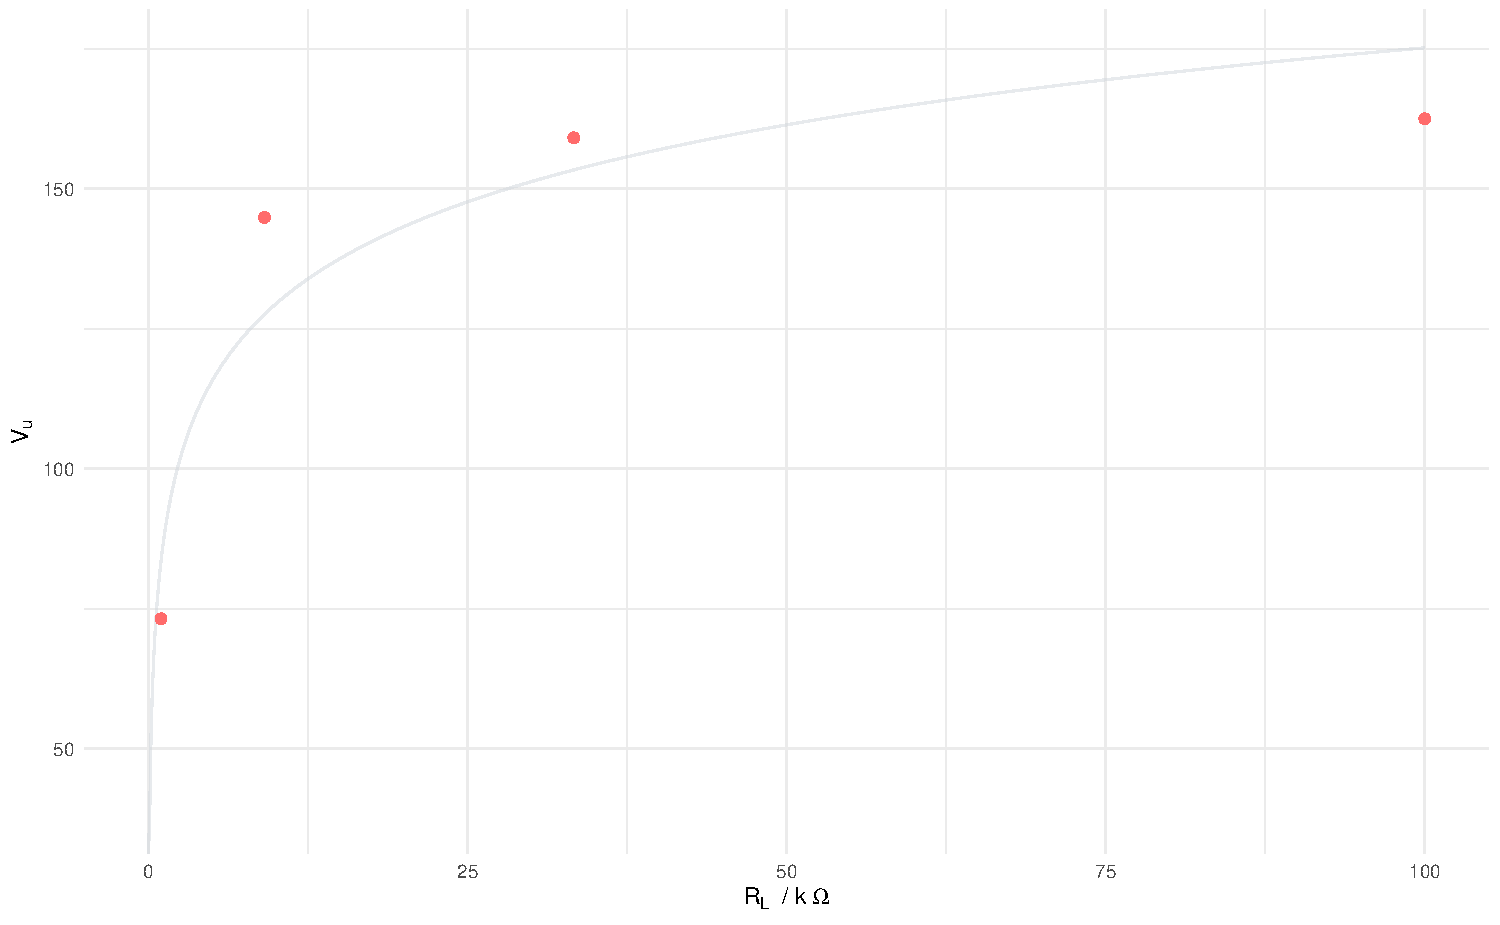
\includegraphics[width=\textwidth]{2_3/2_3_1.pdf}
  \end{center}
  \caption{Graph der Messwerte}
\end{figure}

Der Anstieg des Graphen entspricht der Steilheit $g_m$ des Transistors. Die
Steilheit im Arbeitspunkt ist etwa
\[g_m = \frac{I_C}{U_T} = \frac{4.33 \, \si{\milli\ampere}}{26 \,
    \si{\milli\volt}} = 188.26 \, \si{\milli\siemens}\]

Der theoretische Zusammenhang ist
\[V_u = - g_m \cdot R_L \] 

Der scheinbar lineare Zusammenhang ist aus dem Messwertgraphen jedoch nicht
erkennbar. Dies liegt daran, dass der interne Kollektorwiderstand $R_3$ als
Parallelschaltung in den Gesamtlastwiderstand eingeht.
\[V_u = -g_m \cdot R_3 // R_{\mathrm{L,extern}}\]

$R_3 = 1.3 \, \si{\kilo\ohm}$ legt hier durch die Parallelschaltung den
theoretischen Grenzwert der Spannungsverstärkung fest. \[|V_{u,max}| = 188.26 \,
  \si{\milli\siemens} \cdot 1.3 \, \si{\kilo\ohm} \approx 245\]


Bei hohen externen Widerstandswerten dominiert der Widerstand $R_3$ in der
Parallelschaltung, wodurch der Gesamtlastwiderstand etwa $R_3$ ist, die
Verstärkung läuft gegen einen konstanten Wert.
Bei geringen Widerstandswerten muss die Parallelschaltung berücksichtigt
werden.

Durch Berücksichtung des Kollektorwiderstandes erhält man dann den erwarteten Zusammenhang.

\begin{figure}[H]
  \begin{center}
    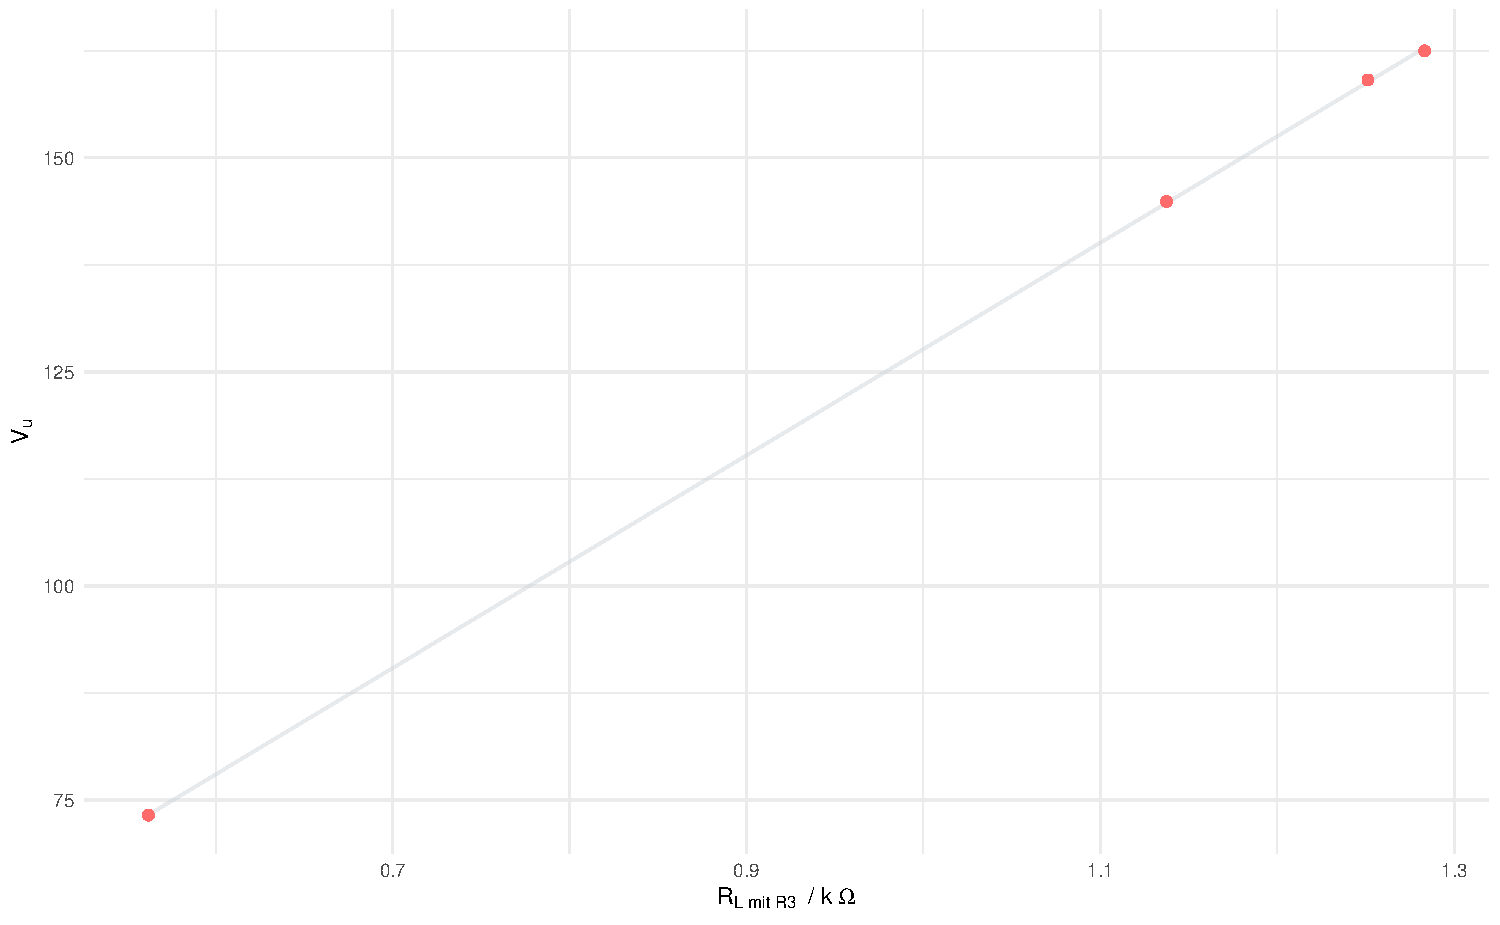
\includegraphics[width=\textwidth]{2_3/2_3_1_corrected.pdf}
  \end{center}
  \caption{Graph der Messwerte, korrigiert}
\end{figure}

Die resultierende Steilheit ist somit:
\[g_m \approx 128 \, \si{\milli\siemens}\]


(Da die Eingangsspannung den Kollektorstrom jedoch etwas verschiebt, ist die
Steilheit nicht konstant, was zu einer Abweichung des theoretisch linearen
Verhaltens führt. Außerdem wurde der Ausgangswiderstand des Transistors nicht berücksichtigt)

\subsubsection{Eingangswiderstand}
Mithilfe der U/2-Methode wurde der Eingangswiderstand der Schaltung bei
konstantem Lastwiderstand von $100 \, \si{\kilo\ohm}$ (kein externer Widerstand)
und einer Frequenz von $1 \, \si{\kilo\hertz}$ bestimmt.

\[U_{a1} = \frac{U_a}{2} = 413 \, \si{\milli\volt}\]

Der dabei ermittelte Eingangswiderstand ist
\[r_e = 800 \, \si{\ohm}\]

\subsubsection{Ausgangswiderstand}
Der Ausgangswiderstand bestimmt sich über die umgestellte Spannungsteilerformel
am Ausgangskreis. $U_{a0}$ ist die Leerlaufspannung, ohne Belastung. $U_{a1}$
die Ausgangsspannung bei Belastung mit $R_L$.
\[U_{a1} = U_{a0} \cdot \frac{R_L}{r_a + R_L}\]
\[r_a = R_L \left( \frac{U_{a0}}{U_{a1}} -1 \right)\]

\[U_{a0} = 821.45 \, \si{\milli\volt}\]
\[U_{a1} = 731.50 \, \si{\milli\volt}\]

\[r_a = 100 \, \si{\kilo\ohm} \left( \frac{ \, \si{\milli\volt}}{\,
      \si{\milli\volt}} -1 \right) = \, \si{\kilo\ohm}\]


\subsubsection{Amplituden-Frequenzgang}
Der Amplituden-Frequenzgang wurde durch das Durchlaufen der
Eingangsspannungsfrequenzen von $0$ bis $10 \, \si{\kilo\hertz}$ und die Messung
der Ausgangsspannungswerte (RMS) bei einer Eingangsspannung von $U_e =
5\,\si{\milli\volt}_{\mathrm{RMS}}$ ermittelt.

\begin{figure}[H]
  \begin{center}
    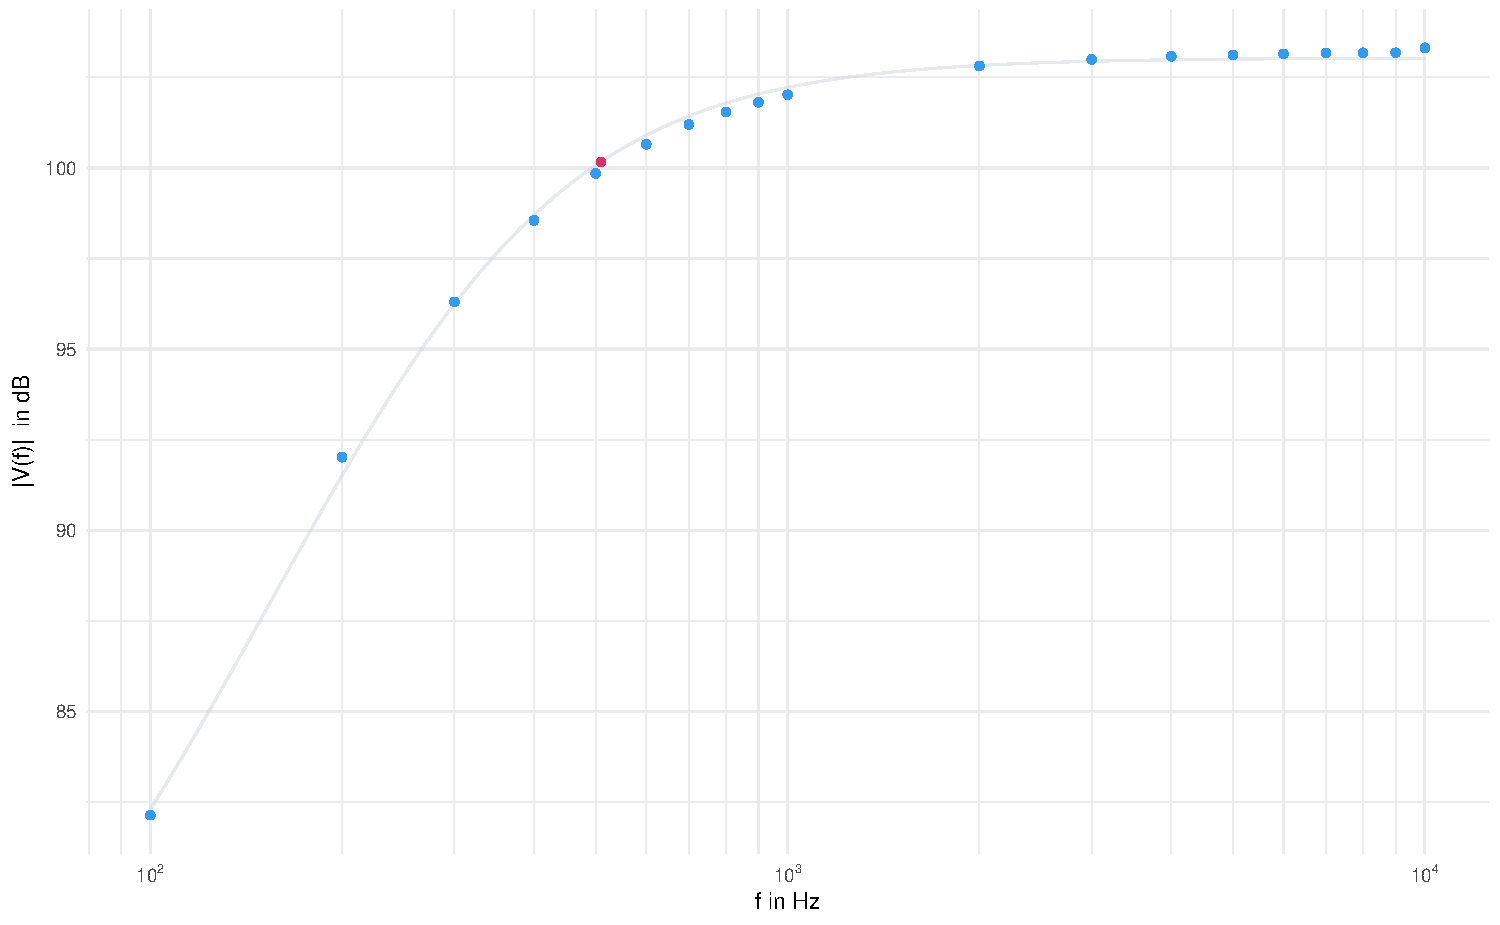
\includegraphics[width=\textwidth]{2_3/2_3_frequenzgang.pdf}
  \end{center}
  \caption{Amplitudenfrequenzgang der Messung}
\end{figure}

Die durch Regression ermittelte Grenzfrequenz ist
\[f_g = 500 \, \si{\hertz}\]

Vor der Grenzfrequenz steigt die Verstärkung mit etwa $25 \, \si{\deci\bel}$ pro
Dekade. Weit hinter der Grenzfrequenz nimmt sie den entsprechenden Wert aus
2.3.1 an.

$C_E$ ($C_3$) stellt wechselstromseitig einen Kurzschluss dar, wodurch der
Emitterwiderstand diesbezüglich wegfällt und die Verstärkung für 
Wechselspannungen deren Frequenz hoch genug ist nicht beeinflusst. Bei
niedrigeren Frequenzen ist die Reaktanz des Kondensators jedoch nicht
ausreichend gering, um den Einfluss von $R_E$ vollständig zu beseitigen.

\end{document}
